\documentclass{article}
\usepackage{fix-cm}
\usepackage{amsmath}
\usepackage{tikz}
\usetikzlibrary{fit}
\usepackage{fancyhdr}
\usepackage{enumitem}
\usepackage[left=2cm, right=2cm, top=4cm, bottom=2cm]{geometry}

\usetikzlibrary{positioning, shapes, arrows.meta, calc}

\setlength{\headheight}{23pt}
\addtolength{\topmargin}{-11pt}

\begin{document}
\title{Derivation of Newton's Law of Gravitation}
\author{Newton, Isaac}
\date{\today}
\maketitle

\begin{abstract}
    This paper is about newton's law of gravitation. It is a very important law in physics. It is given by the formula: $F = \frac{G m_1 m_2}{r^2}$. This law is very important because it explains why objects fall to the ground. It also explains why the moon orbits the earth. It also explains why the earth orbits the sun. It also explains why the planets orbit the sun. It also explains why the sun orbits the center of the galaxy. It also explains why the galaxy orbits the center of the universe. It also explains why the universe is expanding.
\end{abstract}

\section{Introduction}
Newton's law of gravitation is given by the formula:
\[
    F = \frac{G m_1 m_2}{r^2}
\]
where:
\begin{align*}
    F                    & \text{ is the gravitational force between two objects,}      \\
    G                    & \text{ is the gravitational constant,}                       \\
    m_1 \text{ and } m_2 & \text{ are the masses of the two objects, and}               \\
    r                    & \text{ is the separation between the centers of the masses.}
\end{align*}

\subsection{Derivation}
The gravitational force is proportional to the product of the masses and inversely proportional to the square of the separation. We express this relationship as:
\[
    F \propto \frac{m_1 \cdot m_2}{r^2}
\]
Introducing the gravitational constant $G$, we get:
\[
    F = G \cdot \frac{m_1 \cdot m_2}{r^2}
\]
This is the formula for Newton's law of gravitation.

\newpage
\section*{\fontsize{24.88}{30}\selectfont \textbf{About \LaTeX}}

\section*{What is LaTeX and How Does It Work?}

LaTeX is a typesetting system widely used for the preparation of scientific and mathematical documents. It excels in handling complex equations and producing high-quality output. The system works by processing plain text files containing a mixture of formatting commands and regular text. Users create a LaTeX document by writing code that specifies the structure and formatting of the document. The LaTeX system then processes this code to produce a formatted document. The code is typically written in a plain text editor and saved with a \texttt{.tex} file extension.

\begin{figure}[ht]
    \centering
    \begin{tikzpicture}[scale=1.5]
        % Draw the axes
        \draw[->] (-2,0) -- (2,0) node[right] {$x$};
        \draw[->] (0,-2) -- (0,2) node[above] {$y$};

        % Define the function
        \def\func(#1,#2){2*#1*#2^3 + #1^3 + #1^2*#2 + 2}

        % Draw the graph
        \draw[domain=-1.5:1.5, smooth, variable=\x, thick] plot ({\x},{\func(\x,0)});
    \end{tikzpicture}
    \caption{Graph of the function $y = 2xy^3 + x^3 + x^2y + 2$}
\end{figure}

\newpage
\section*{Types of Neural Network Models}

\begin{enumerate}[label=\arabic*.]

    \item \textbf{Feedforward Neural Networks (FNN):}

          Basic neural network architecture where information travels in one direction, from the input layer to the output layer. Often used for simple classification tasks.

          \begin{figure}[ht]
              \centering
              \begin{tikzpicture}
                  % Nodes
                  \foreach \i in {1,2,3}
                  \node[circle, draw, minimum size=8mm] (input\i) at (0,-\i) {$x_{\i}$};
                  \node[circle, draw, minimum size=8mm] (output) at (2,-2) {$y$};

                  % Arrows
                  \foreach \i in {1,2,3}
                  \draw[->] (input\i) -- (output);
              \end{tikzpicture}
              \caption{Feedforward Neural Network}
          \end{figure}

    \item \textbf{Multilayer Perceptrons (MLP):}

          An extension of feedforward neural networks with one or more hidden layers between the input and output layers. Widely used for various applications, including image recognition and natural language processing.

          \begin{figure}[ht]
              \centering
              \begin{tikzpicture}
                  % Nodes
                  \foreach \i in {1,2,3}
                  \node[circle, draw, minimum size=8mm] (input\i) at (0,-\i) {$x_{\i}$};
                  \foreach \h in {1,2}
                  \node[circle, draw, minimum size=8mm, yshift=-1cm] (hidden\h) at (2,-\h) {$h_{\h}$};
                  \node[circle, draw, minimum size=8mm] (output) at (4,-2.5) {$y$};

                  % Arrows
                  \foreach \i in {1,2,3}
                  \foreach \h in {1,2}
                  \draw[->] (input\i) -- (hidden\h);
                  \foreach \h in {1,2}
                  \draw[->] (hidden\h) -- (output);
              \end{tikzpicture}
              \caption{Multilayer Perceptron}
          \end{figure}

    \item \textbf{Convolutional Neural Networks (CNN):}

          Specifically designed for image recognition and processing. Uses convolutional layers to automatically and adaptively learn spatial hierarchies of features.

          \begin{figure}[ht]
              \centering
              \begin{tikzpicture}
                  % Input
                  \draw (0,0) grid (4,4) {};
                  \foreach \x in {0,1,2,3}
                  \foreach \y in {0,1,2,3}
                  \node at (\x+0.5, \y+0.5) {(\x,\y)};
                  \node at (2, -0.5) {Input Image};

                  % Convolutional Layer
                  \foreach \x in {0,1,2,3}
                  \foreach \y in {0,1,2,3}
                  \node[minimum size=7mm, draw] (conv\y\x) at (5+\x, .5+\y) {$\x\y$};
                  \node at (6.5, -0.5) {Convolutional Layer};

                  \foreach \i in {0,2}
                  \foreach \j in {0,2}
                  \node[draw, dashed, inner sep=0.6mm, fit=(conv\i\j) (conv\i\the\numexpr\j+1\relax) (conv\the\numexpr\i+1\relax\j) (conv\the\numexpr\i+1\relax\the\numexpr\j+1\relax)] (group\the\numexpr\i/2\relax\the\numexpr\j/2\relax) {};

                  % Pooling Layer
                  \foreach \x in {0,1}
                  \foreach \y in {0,1}
                  \node[minimum size=8mm, draw] (pool\y\x) at (10+\x, 1.5+\y) {$\x\y$};
                  \node at (10.5, 0.5) {Pooling Layer};

                  % Output Layer
                  \node[minimum size=8mm, draw] (output) at (13, 2) {$\delta$};
                  \node at (13, 1) {Output};

                  % Arrows
                  \foreach \i in {0,1}
                  \foreach \j in {0,1}
                  \pgfmathsetmacro{\k}{\j/2}
                  \draw[->, blue, line width=1pt] (group\i\j) -- (pool\i\j);


                  \foreach \i in {0,1}
                  \foreach \j in {0,1}
                  \draw[->, red, line width=1pt]  (pool\i\j) -- (output);


              \end{tikzpicture}
              \caption{Convolutional Neural Network}
          \end{figure}

    \item \textbf{Recurrent Neural Networks (RNN):}

          Suitable for sequential data, such as time series or natural language. Has connections that form a directed cycle, allowing information persistence.

          \begin{figure}[ht]
              \centering
              \begin{tikzpicture}
                  % Nodes
                  \foreach \i in {1,2,3}
                  \node[circle, draw, minimum size=8mm] (input\i) at (0,-\i) {$x_{\i}$};
                  \foreach \h in {1,2,3}
                  \node[circle, draw, minimum size=8mm, yshift=-1cm] (hidden\h) at (2,-\h) {$h_{\h}$};
                  \node[circle, draw, minimum size=8mm] (output) at (4,-2.5) {$y$};

                  % Arrows
                  \foreach \i in {1,2,3}
                  \foreach \h in {1,2,3}
                  \draw[->] (input\i) -- (hidden\h);
                  \foreach \h in {1,2,3}
                  \draw[->] (hidden\h) -- (output);
                  \foreach \h/\i in {1/1,2/2,3/3}
                  \draw[->] (hidden\h) to[out=135,in=45] (hidden\i);
              \end{tikzpicture}
              \caption{Recurrent Neural Network}
          \end{figure}

    \item \textbf{Long Short-Term Memory (LSTM):}

          A type of RNN with memory cells that can store information for long periods, preventing the vanishing gradient problem. Effective for learning and remembering over long sequences.

          \begin{figure}[ht]
              \centering
              \begin{tikzpicture}
                  % Nodes
                  \foreach \i in {1,2,3}
                  \node[circle, draw, minimum size=8mm] (input\i) at (0,-\i) {$x_{\i}$};
                  \foreach \h in {1,2,3}
                  \node[rectangle, draw, minimum size=8mm, yshift=-1cm] (cell\h) at (2,-\h) {$c_{\h}$};
                  \node[circle, draw, minimum size=8mm] (output) at (4,-2.5) {$y$};

                  % Arrows
                  \foreach \i in {1,2,3}
                  \foreach \h in {1,2,3}
                  \draw[->] (input\i) -- (cell\h);
                  \foreach \h in {1,2,3}
                  \draw[->] (cell\h) -- (output);
                  \foreach \h/\i in {1/1,2/2,3/3}
                  \draw[->] (cell\h) to[out=135,in=45] (cell\i);
              \end{tikzpicture}
              \caption{Long Short-Term Memory (LSTM)}
          \end{figure}

    \item \textbf{Gated Recurrent Unit (GRU):}

          Similar to LSTM but with a simpler architecture. Efficient in capturing dependencies in sequential data.
          \begin{figure}[ht]
              \centering
              \begin{tikzpicture}
                  % Nodes
                  \foreach \i in {1,2,3}
                  \node[circle, draw, minimum size=8mm] (input\i) at (0,-\i) {$x_{\i}$};
                  \foreach \h in {1,2,3}
                  \node[circle, draw, minimum size=8mm, yshift=-1cm] (hidden\h) at (2,-\h) {$h_{\h}$};
                  \node[circle, draw, minimum size=8mm] (output) at (4,-2.5) {$y$};

                  % Arrows
                  \foreach \i in {1,2,3}
                  \foreach \h in {1,2,3}
                  \draw[->] (input\i) -- (hidden\h);
                  \foreach \h in {1,2,3}
                  \draw[->] (hidden\h) -- (output);
                  \foreach \h/\i in {1/1,2/2,3/3}
                  \draw[->] (hidden\h) to[out=135,in=45] (hidden\i);
                  \foreach \i in {1,2,3}
                  \draw[->] (hidden\i) to[out=-45,in=-135] (output);
              \end{tikzpicture}
              \caption{Gated Recurrent Unit (GRU)}
          \end{figure}

          \newpage
    \item \textbf{Autoencoders:}

          Unsupervised learning models that aim to learn efficient representations of input data. Consists of an encoder that maps input data to a lower-dimensional representation and a decoder that reconstructs the input from this representation.
          \begin{figure}[ht]
              \centering
              \begin{tikzpicture}
                  % Nodes
                  \foreach \i in {1,2,3}
                  \node[circle, draw, minimum size=8mm] (input\i) at (0,-\i) {$x_{\i}$};
                  \foreach \h in {1,2}
                  \node[circle, draw, minimum size=8mm, yshift=-1cm] (hidden\h) at (2,-\h) {$h_{\h}$};
                  \foreach \i in {1,2,3}
                  \node[circle, draw, minimum size=8mm, yshift=-2cm] (output\i) at (4,-\i) {$\hat{x}_{\i}$};

                  % Arrows
                  \foreach \i in {1,2,3}
                  \foreach \h in {1,2}
                  \draw[->] (input\i) -- (hidden\h);
                  \foreach \h in {1,2}
                  \foreach \i in {1,2,3}
                  \draw[->] (hidden\h) -- (output\i);
              \end{tikzpicture}
              \caption{Autoencoders}
          \end{figure}

    \item \textbf{Generative Adversarial Networks (GAN):}

          Comprises a generator and a discriminator trained simultaneously through adversarial training. Used for generating new data that is similar to a given dataset.
          \begin{figure}[ht]
              \centering
              \begin{tikzpicture}
                  % Nodes
                  \node[rectangle, draw, minimum size=8mm] (generator) at (0,0) {Generator};
                  \node[rectangle, draw, minimum size=8mm] (discriminator) at (4,0) {Discriminator};

                  % Arrows
                  \draw[->] (generator) -- node[above] {$G(z)$} (discriminator);
                  \draw[->] ([yshift=-5mm]discriminator.south) -- node[below] {$D(x)$} ([yshift=-5mm]generator.south);
              \end{tikzpicture}
              \caption{Generative Adversarial Networks (GAN)}
          \end{figure}

    \item \textbf{Radial Basis Function Networks (RBFN):}

          Utilizes radial basis functions as activation functions. Commonly used for function approximation and pattern recognition.
          \begin{figure}[ht]
              \centering
              \begin{tikzpicture}
                  % Nodes
                  \foreach \i in {1,2,3}
                  \node[circle, draw, minimum size=8mm] (input\i) at (0,-\i) {$x_{\i}$};
                  \foreach \h in {1,2,3}
                  \node[circle, draw, minimum size=8mm, yshift=-1cm] (hidden\h) at (2,-\h) {$\phi_{\h}$};
                  \node[circle, draw, minimum size=8mm] (output) at (4,-2.5) {$y$};

                  % Arrows
                  \foreach \i in {1,2,3}
                  \foreach \h in {1,2,3}
                  \draw[->] (input\i) -- (hidden\h);
                  \foreach \h in {1,2,3}
                  \draw[->] (hidden\h) -- (output);
              \end{tikzpicture}
              \caption{Radial Basis Function Networks (RBFN)}
          \end{figure}

          \newpage
    \item \textbf{Self-Organizing Maps (SOM):}

          Unsupervised learning models that map input data into a lower-dimensional grid while preserving the topological properties of the input space. Useful for clustering and visualization.
          \begin{figure}[ht]
              \centering
              \begin{tikzpicture}
                  % Nodes
                  \foreach \i in {1,2,3}
                  \node[circle, draw, minimum size=8mm] (input\i) at (0,-\i) {$x_{\i}$};
                  \node[ellipse, draw, minimum size=8mm] (output) at (4,-2.5) {Winner};

                  % Arrows
                  \foreach \i in {1,2,3}
                  \draw[->] (input\i) -- (output);
              \end{tikzpicture}
              \caption{Self-Organizing Maps (SOM)}
          \end{figure}

    \item \textbf{Hopfield Networks:}

          A type of recurrent neural network used for associative memory and pattern recognition. Can store and recall patterns even if they are partially corrupted.
          \begin{figure}[ht]
              \centering
              \begin{tikzpicture}
                  % Nodes
                  \foreach \i in {1,2,3}
                  \node[circle, draw, minimum size=8mm] (input\i) at (0,-\i) {$x_{\i}$};
                  \foreach \h in {1,2,3}
                  \node[circle, draw, minimum size=8mm, yshift=-1cm] (memory\h) at (2,-\h) {$m_{\h}$};
                  \node[circle, draw, minimum size=8mm] (output) at (4,-2.5) {$y$};

                  % Arrows
                  \foreach \i in {1,2,3}
                  \foreach \h in {1,2,3}
                  \draw[->] (input\i) -- (memory\h);
                  \foreach \h in {1,2,3}
                  \draw[->] (memory\h) -- (output);
                  \foreach \h/\i in {1/1,2/2,3/3}
                  \draw[->] (memory\h) to[out=135,in=45] (memory\i);
              \end{tikzpicture}
              \caption{Hopfield Networks}
          \end{figure}

    \item \textbf{Neural Turing Machines (NTM):}

          Integrates the capabilities of a traditional Turing machine with a neural network. Enables learning and reasoning algorithmic tasks.

          \begin{figure}[ht]
              \centering
              \begin{tikzpicture}
                  % Nodes
                  \foreach \i in {1,2,3}
                  \node[circle, draw, minimum size=8mm] (input\i) at (0,-\i) {$x_{\i}$};
                  \foreach \h in {1,2,3}
                  \node[rectangle, draw, minimum size=8mm, yshift=-1cm] (memory\h) at (2,-\h) {$m_{\h}$};
                  \node[circle, draw, minimum size=8mm] (output) at (4,-2.5) {$y$};

                  % Arrows
                  \foreach \i in {1,2,3}
                  \foreach \h in {1,2,3}
                  \draw[->] (input\i) -- (memory\h);
                  \foreach \h in {1,2,3}
                  \draw[->] (memory\h) -- (output);
                  \foreach \h/\i in {1/1,2/2,3/3}
                  \draw[->] (memory\h) to[out=135,in=45] (memory\i);
                  \foreach \i in {1,2,3}
                  \draw[->] (memory\i) to[out=-45,in=-135] (output);
              \end{tikzpicture}
              \caption{Neural Turing Machines (NTM)}
          \end{figure}

          \newpage
    \item \textbf{Transformers:}

          Originally designed for natural language processing, especially for sequence-to-sequence tasks. Self-attention mechanism allows the model to weigh different parts of the input sequence differently.

          \begin{figure}[ht]
              \centering
              \begin{tikzpicture}
                  % Nodes
                  \foreach \i in {1,2,3}
                  \node[circle, draw, minimum size=8mm] (input\i) at (0,-\i) {$x_{\i}$};
                  \foreach \h in {1,2,3}
                  \node[rectangle, draw, minimum size=8mm, yshift=-1cm] (memory\h) at (2,-\h) {$m_{\h}$};
                  \node[circle, draw, minimum size=8mm] (output) at (4,-2.5) {$y$};

                  % Arrows
                  \foreach \i in {1,2,3}
                  \foreach \h in {1,2,3}
                  \draw[->] (input\i) -- (memory\h);
                  \foreach \h in {1,2,3}
                  \draw[->] (memory\h) -- (output);
                  \foreach \i in {1,2,3}
                  \draw[->] (memory\i) to[out=-45,in=-135] (output);
                  \draw[dashed, ->] (input1) -- (input3) node[midway, left, xshift=-1cm] {Self-Attention};
              \end{tikzpicture}
              \caption{Transformers}
          \end{figure}

\end{enumerate}
\end{document}
